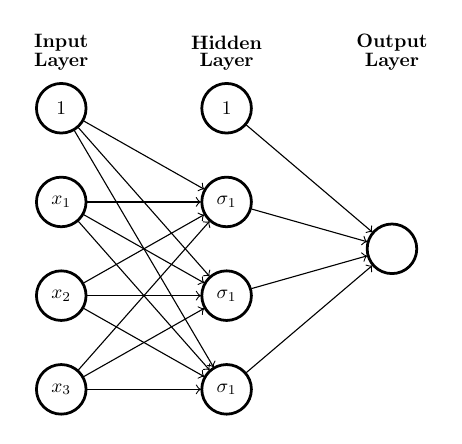
\begin{tikzpicture}[scale=0.7, every node/.style={scale=0.7}]
    %--------------------%
    % Parameters
    %--------------------%
    \def\layersep{3}
    \def\ysep{1.7}
    \def\circlesize{0.9cm}
    \def\labelshift{0.75}
    \def\woffset{5}
    \def\linethic{1.0pt}

    %--------------------%
    % Input Layer
    %--------------------%

    \node[draw, circle, minimum size=\circlesize, line width=\linethic] (theta0) at (0,2*\ysep) {1};
    \node[draw ,circle, minimum size=\circlesize, line width=\linethic] (x1) at (0,1*\ysep) {$x_1$};
    \node[draw ,circle, minimum size=\circlesize, line width=\linethic] (x2) at (0,0*\ysep) {$x_2$};
    \node[draw ,circle, minimum size=\circlesize, line width=\linethic] (x3) at (0,-1*\ysep) {$x_3$};

    %--------------------%
    % Layer 1
    %--------------------%
    % Nodes
    \node[draw, circle, minimum size=\circlesize, line width=\linethic] (theta1) at (\layersep,2*\ysep) {1};
    \node[draw ,circle, minimum size=\circlesize, line width=\linethic] (node1) at (\layersep,1*\ysep) {$\sigma_{1}$};
    \node[draw ,circle, minimum size=\circlesize, line width=\linethic] (node2) at (\layersep,0*\ysep) {$\sigma_{1}$};
    \node[draw ,circle, minimum size=\circlesize, line width=\linethic] (node3) at (\layersep,-1*\ysep) {$\sigma_{1}$};


    %--------------------%
    % Output Layer
    %--------------------%
    \node[draw ,circle, minimum size=\circlesize, line width=\linethic] (out) at (2*\layersep,0.5*\ysep) {};

    %--------------------%
    % Connections
    %--------------------%
    % Input to Layer 1
    \draw[->] (theta0) -- node[above,midway]{} (node1);
    \draw[->] (theta0) -- node[above,midway]{} (node2);
    \draw[->] (theta0) -- node[above,midway]{} (node3);
    \draw[->] (x1) -- node[above,midway]{} (node1);
    \draw[->] (x1) -- node[above,midway]{} (node2);
    \draw[->] (x1) -- node[above,midway]{} (node3);
    \draw[->] (x2) -- node[above,midway]{} (node1);
    \draw[->] (x2) -- node[above,midway]{} (node2);
    \draw[->] (x2) -- node[above,midway]{} (node3);
    \draw[->] (x3) -- node[above,midway]{} (node1);
    \draw[->] (x3) -- node[above,midway]{} (node2);
    \draw[->] (x3) -- node[above,midway]{} (node3);

   % Layer 2 to Output Layer
    \draw[->] (theta1) -- node[above,midway]{} (out);
    \draw[->] (node1) -- node[above,midway]{} (out);
    \draw[->] (node2) -- node[above,midway]{} (out);
    \draw[->] (node3) -- node[above,midway]{} (out);


    %--------------------%
    % Layer Labels
    %--------------------%
    \node at (0*\layersep, 2.7*\ysep) {\textbf{Input}};
    \node at (0*\layersep, 2.5*\ysep) {\textbf{Layer}};
    \node at (1*\layersep, 2.7*\ysep) {\textbf{Hidden}};
    \node at (1*\layersep, 2.5*\ysep) {\textbf{Layer}};
    \node at (2*\layersep, 2.7*\ysep) {\textbf{Output}};
    \node at (2*\layersep, 2.5*\ysep) {\textbf{Layer}};

\end{tikzpicture}
